\documentclass[tikz,border=8pt]{standalone}
\usepackage[T1]{fontenc}
\usepackage{helvet}
\renewcommand{\familydefault}{\sfdefault}
\usepackage{xcolor}
\usetikzlibrary{arrows.meta,positioning,calc,fit,backgrounds}

\definecolor{Navy}{HTML}{26418F}
\definecolor{Green}{HTML}{86BC25}
\definecolor{Burgundy}{HTML}{B5121B}
\definecolor{LightGray}{HTML}{F2F2F2}
\definecolor{DarkGray}{HTML}{44546A}
\definecolor{MidGray}{HTML}{D9D9D9}

\tikzset{
  box/.style={
    rounded corners=6pt,
    draw=#1,
    very thick,
    fill=white,
    text=DarkGray,
    align=center,
    text width=4.45cm,
    inner xsep=8pt,
    inner ysep=10pt,
    minimum width=4.95cm,
    minimum height=1.70cm,
    font=\footnotesize
  },
  titlebox/.style={
    font=\bfseries\footnotesize,
    text=white,
    fill=#1,
    rounded corners=4pt,
    inner xsep=6pt,
    inner ysep=3pt
  },
  layerlabel/.style={
    font=\bfseries\scriptsize,
    text=#1,
    align=left
  },
  flowarrow/.style={
    -{Stealth[length=3.0mm,width=2.0mm]},
    very thick,
    draw=DarkGray,
    rounded corners=7pt,
    shorten <=2pt,
    shorten >=2pt
  },
  softpanel/.style={
    rounded corners=8pt,
    fill=LightGray,
    draw=MidGray,
    line width=0.4pt
  }
}

\newcommand{\workflowbox}[5]{%
  \node[box=#4] (#1) at (#2) {%
    #5
  };
  \node[titlebox=#4, anchor=south] at ([yshift=2.5pt]#1.north) {#3};
}

\begin{document}
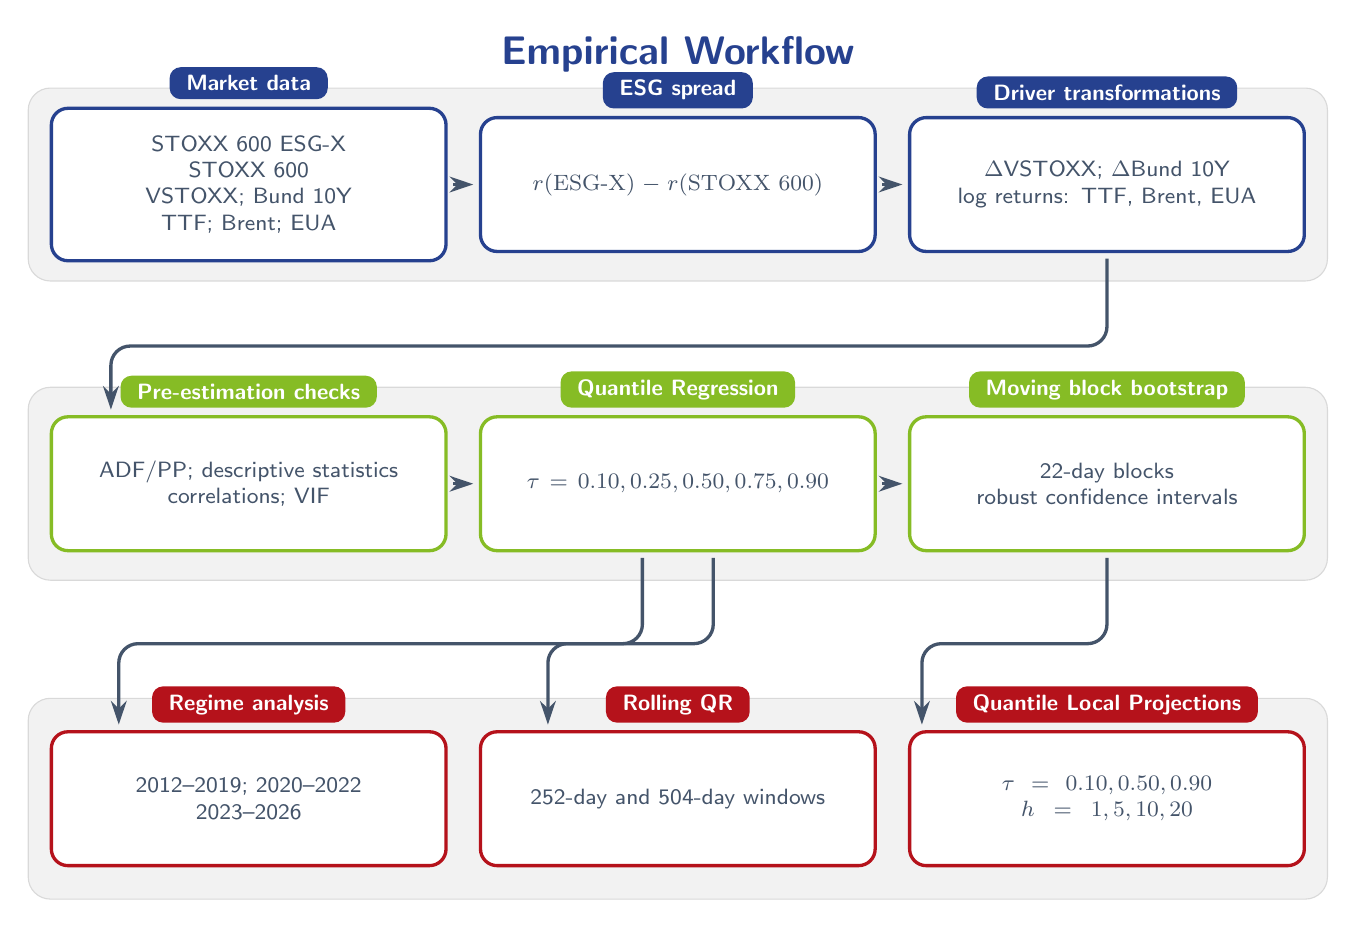
\begin{tikzpicture}[x=1cm,y=1cm]

% Background layer panels.
\begin{scope}[on background layer]
  \node[softpanel, minimum width=16.5cm, minimum height=2.45cm] at (0, 4.25) {};
  \node[softpanel, minimum width=16.5cm, minimum height=2.45cm] at (0, 0.45) {};
  \node[softpanel, minimum width=16.5cm, minimum height=2.55cm] at (0,-3.55) {};
\end{scope}

% Main title.
\node[font=\bfseries\Large, text=Navy] at (0,5.90) {Empirical Workflow};

% Layer 1: data and variable construction.
\workflowbox{market}{-5.45,4.25}{Market data}{Navy}{%
  STOXX 600 ESG-X\\
  STOXX 600\\
  VSTOXX; Bund 10Y\\
  TTF; Brent; EUA}

\workflowbox{spread}{0,4.25}{ESG spread}{Navy}{%
  \(r(\mathrm{ESG\mbox{-}X}) - r(\mathrm{STOXX\ 600})\)}

\workflowbox{drivers}{5.45,4.25}{Driver transformations}{Navy}{%
  \(\Delta\)VSTOXX; \(\Delta\)Bund 10Y\\
  log returns: TTF, Brent, EUA}

% Layer 2: baseline econometric framework.
\workflowbox{checks}{-5.45,0.45}{Pre-estimation checks}{Green}{%
  ADF/PP; descriptive statistics\\
  correlations; VIF}

\workflowbox{qr}{0,0.45}{Quantile Regression}{Green}{%
  \(\tau = 0.10, 0.25, 0.50, 0.75, 0.90\)}

\workflowbox{boot}{5.45,0.45}{Moving block bootstrap}{Green}{%
  22-day blocks\\
  robust confidence intervals}

% Layer 3: heterogeneity and dynamics.
\workflowbox{regime}{-5.45,-3.55}{Regime analysis}{Burgundy}{%
  2012--2019; 2020--2022\\
  2023--2026}

\workflowbox{rolling}{0,-3.55}{Rolling QR}{Burgundy}{%
  252-day and 504-day windows}

\workflowbox{qlp}{5.45,-3.55}{Quantile Local Projections}{Burgundy}{%
  \(\tau = 0.10, 0.50, 0.90\)\\
  \(h = 1, 5, 10, 20\)}

% Arrows within layers.
\draw[flowarrow] (market.east) -- (spread.west);
\draw[flowarrow] (spread.east) -- (drivers.west);
\draw[flowarrow] (drivers.south) -- ++(0,-1.18)
  -| ([xshift=-1.75cm]checks.north);

\draw[flowarrow] (checks.east) -- (qr.west);
\draw[flowarrow] (qr.east) -- (boot.west);

% Split from baseline framework to robustness and dynamics.
\draw[flowarrow] ([xshift=-0.45cm]qr.south) -- ++(0,-1.16)
  -| ([xshift=-1.65cm]rolling.north);
\draw[flowarrow] (boot.south) -- ++(0,-1.16)
  -| ([xshift=-2.35cm]qlp.north);
\draw[flowarrow] ([xshift=0.45cm]qr.south) -- ++(0,-1.16)
  -| ([xshift=-1.65cm]regime.north);

\end{tikzpicture}
\end{document}
